\section{Fourier Series}
\begin{itemize}
    \item Fourier Series is used to represent periodic functions using a series consisting of trigonometric functions.
    \begin{definition}
        A function is periodic if and only if there exists a constant $T$ such that $f(t+T)=f(t)$. The smallest positive value $T$ is known as the fundamental period.
    \end{definition} 
    \begin{example}
        If we have a function in the form of: 
        \begin{equation}
            f(t) = \cos(\pi t) + \frac{1}{2}\sin(2\pi t)
            \label{eqn:fourier}
        \end{equation}
        The period of the first term is $2$ and the period of the second term is $1$. The smallest period for $f$ is $2$:
\begin{example}
    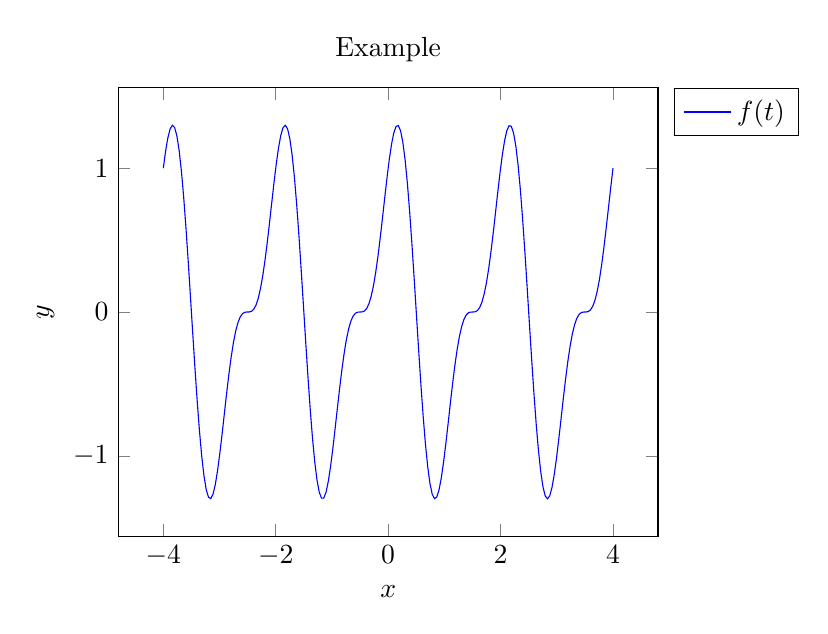
\begin{tikzpicture}
        \begin{axis}[
        legend pos=outer north east,
        title=Example,
        axis lines = box,
        xlabel = $x$,
        ylabel = $y$,
        variable = t,
        trig format plots = rad,
        ]
        \addplot [
            domain=-4:4,
            samples=200,
            color=blue,
            ]
            {cos(pi*x)+0.5*sin(2*pi*x)};
        \addlegendentry{$f(t)$}
        \end{axis}
        \end{tikzpicture}
\end{example}
    \end{example}
    \begin{theorem}
        For $f(t)$ periodic, with fundamental period $T$, continuous and piecewise differentiable, then:
        \begin{equation}
            f(t)=\frac{a_0}{2}+\sum_{n=1}^\infty a_n\cos (n\omega t) + b_n\sin(n\omega t)
        \end{equation}
        where $\omega = \frac{2\pi}{T}$ is known as the Fourier series of $f$. $a_n$ and $b_n$ are Fourier coefficients.
    \end{theorem}
    \item To determine the coefficients, we need the following integrals:
    \begin{equation}
        \int_{-T/2}^{T/2} \cos(n\omega t)\dd{t} = \begin{cases}
            0 & n\neq 0 \\ 
            T & n=0
        \end{cases}
    \end{equation}
    \begin{equation}
        \int_{-T/2}^{T/2}\sin(n\omega t)\dd{t} = 0
    \end{equation}
    \begin{equation}
        \int_{-T/2}^{T/2}\cos(m\omega t)\cos(n\omega t)\dd{t} = \begin{cases}
            0 & m\neq n \\ 
            T/2 & m=n
        \end{cases}
    \end{equation}
    % \begin{equation}
    %     \int_{-T/2}^{T/2} \cos(m\omega t)\sin(n\omega t)\dd{t} =0 
    % \end{equation}
    \begin{example}
        Take the integral $\int_{-T/2}^{T/2} \cos(5\omega t)\cos(3\omega t)\dd{t}$. We can write this as:
        \begin{align}
            &= \frac{1}{2}\int_{-T/2}^{T/2}(\cos(2\omega t) + \cos(8\omega t))\dd{t} \\ 
            &= \frac{1}{2}\left[\frac{1}{2\omega} \sin(2\omega t) + \frac{1}{8\omega}\sin(8\omega t)\right]^{T/2}_{-T/2} \\ 
            &= 0
        \end{align}
    \end{example}
    \item Consider the integrals:
    \begin{align}
        \int_{-T/2}^{T/2} f(t)\cos(m\omega t) \dd{t} &= \frac{T}{2}a_m \\ 
        \int_{-T/2}^{T/2} f(t)\sin(m\omega t) \dd{t} &= \frac{T}{2}b_m 
    \end{align}pi/
    where we have substituted in equation \ref{eqn:fourier} alongside the above integral identities. This then gives the coefficients as:
    \begin{align}
        a_n &= \frac{2}{T}\int_{-T/2}^{T/2} f(t)\cos(n\omega t)\dd{t} \\ 
        b_n &= \frac{2}{T}\int_{-T/2}^{T/2} f(t)\sin(n\omega t)\dd{t}
    \end{align}
    for $n=1,2,3,\dots$.
    \begin{example}
        Suppose we have a triangle function: $f(t)=\pi - t$ from $[-\pi,\pi]$:
        \begin{center}
            \begin{tikzpicture}
                \begin{axis}[
                legend pos=outer north east,
                title=Triangle Function,
                axis lines = box,
                xlabel = $x$,
                ylabel = $y$,
                variable = t,
                trig format plots = rad,
                ]
                \addplot [
                    domain=-pi:pi,
                    samples=70,
                    color=blue,
                    ]
                    {pi-abs(t)};
                \addlegendentry{$\pi - |t|$}
                
                \end{axis}
                \end{tikzpicture}
        \end{center}

        We start by calculating the $b$ coefficient:
        \begin{align}
            b_n &= \frac{2}{2\pi} \int_{-\pi}^{\pi} f(t) \sin(nt) \dd{t} \\ 
            &= \frac{1}{\pi}\int_{-\pi}^{\pi} \pi \sin(nt) \dd{t} - \frac{1}{\pi}(-t)\int_{-\pi}^{\pi}\sin (nt) \dd{t}
        \end{align}
        Notice that since this is an odd function, we have $b_n=0$. Next, we calcluate $a_n$:
        \begin{align}
            a_n &= \frac{2}{2\pi}\int_{-\pi}^{\pi} f(t) \cos(nt) \dd{t} \\ 
            &= 2\frac{1}{\pi} \int_0^{\pi}(\pi -t)\cos(nt) \dd{t} \\ 
            &= \begin{cases}
                \pi & n=0 \\ 
                0 & n\neq 0,\,\text{n is even} \\ 
                \frac{4}{\pi n^2} & \neq 0,\,\text{n is odd}
            \end{cases}
        \end{align}
        Therefore, we have:
        \begin{equation}
            f(t) = \frac{\pi}{2} + \sum_{n=0}^\infty \frac{4}{\pi (2k-1)^2}
        \end{equation}
    \end{example}
    \begin{idea}
        It is helpful to look if the function is even or odd at the beginning, allowing us to immediately set $a_n=0$ or $b_n=0$.
    \end{idea}
    \begin{example}
        Suppose we wish to write the Fourier series of $f(x)=x^2$ from $-\pi \le x \le \pi$. The period is $T=2\pi$ and $\omega = \frac{2\pi}{T}=1$. We then have:
        \begin{align}
            a_n &= \frac{2}{2\pi} \int_{-\pi}^{\pi} t&2 \cos(nt) \dd{t}
        \end{align}
        For $n=0$ we have:
        \begin{equation}
            a_0 = \frac{1}{\pi}\int_{-\pi}^{\pi} t^2 \dd{t} = \frac{2\pi^2}{3}
        \end{equation}
        For $n\neq 0$, we have:
        \begin{align}
            a_n &= \frac{1}{\pi}\int_{-\pi}^{\pi} t^2\cos(nt)\dd{t} \\ 
            &= \frac{1}{\pi n^2}\int_{-\pi}^{\pi} (nt)^2 \cos(nt) \dd{(nt)} \\ 
            &= \frac{1}{\pi n^2}\left[(nt)^2\sin(nt)\right]\Biggr|^{t=\pi}_{t=-\pi}-\frac{2}{\pi n^2}\int_{-\pi}^{\pi} (nt)\sin(nt)\dd{(nt)} & \text{(reduction)} \\ 
            &= -\frac{2}{\pi n^3}(\sin(nt)-nt\cos(nt))\Biggr|^{t=\pi}_{t=-\pi} & \text{(by parts)} \\ 
            &= \begin{cases}
                -\frac{4}{n^2} & \text{n odd} \\ 
                +\frac{4}{n^2} & \text{n even}
            \end{cases}
        \end{align}
        Since the function is even, we have $b_n=0$. Thus:
        \begin{equation}
            f = \frac{\pi^2}{3} + \sum_{n=1}^\infty \frac{4}{n^2}(-1)^{n} \cos nt
        \end{equation}
    \end{example}
\end{itemize}